% 
%            ,,                                        
%          `7MM            _.o9                                
%            MM                                             
%  ,6"Yb.    MM  ,p6"bo   ,6"Yb.  M"""MMV  ,6"Yb.  `7Mb,od8 
% 8)   MM    MM 6M'  OO  8)   MM  '  AMV  8)   MM    MM' "' 
%  ,pm9MM    MM 8M        ,pm9MM    AMV    ,pm9MM    MM     
% 8M   MM    MM YM.    , 8M   MM   AMV  , 8M   MM    MM     
% `Moo9^Yo..JMML.YMbmd'  `Moo9^Yo.AMMmmmM `Moo9^Yo..JMML.   
% 
% 
% Free and Open-Source template for academic works
% https://github.com/dpmj/alcazar



% ------------------------------------------------------------------------------
% FILES

% Title page
% 
%            ,,                                        
%          `7MM            _.o9                                
%            MM                                             
%  ,6"Yb.    MM  ,p6"bo   ,6"Yb.  M"""MMV  ,6"Yb.  `7Mb,od8 
% 8)   MM    MM 6M'  OO  8)   MM  '  AMV  8)   MM    MM' "' 
%  ,pm9MM    MM 8M        ,pm9MM    AMV    ,pm9MM    MM     
% 8M   MM    MM YM.    , 8M   MM   AMV  , 8M   MM    MM     
% `Moo9^Yo..JMML.YMbmd'  `Moo9^Yo.AMMmmmM `Moo9^Yo..JMML.   
% 
% 
% Free and Open-Source template for academic works
% https://github.com/dpmj/alcazar


% ------------------------------------------------------------------------------
% Title page

\thispagestyle{empty}

\pagenumbering{roman}
\setcounter{page}{1}


\newgeometry{
    left    = 3.0cm,
    right   = 3.0cm,
    top     = 3.5cm,
    bottom  = 3.5cm
}


\begin{center}
    
\includegraphics[height=15mm]{opening/resources/logos/logo_upv.pdf}
    \hfill
    
\includegraphics[height=15mm]{opening/resources/logos/logo_upv_telcom.pdf}
\end{center}

\vspace*{30mm}

\begin{center}
    \textbf{\large \textsc{{\thesisDegree} in}}
\end{center}

\vspace*{0mm}

\begin{center}
    \textbf{\large \thesisType}
\end{center}

\vspace*{10mm}

\begin{center}
    \setstretch{1.7}
    \textbf{{\LARGE {}``\thesisTitle''}}\\
\end{center}

\vspace*{15mm}

\begin{center}
    {\large \textsc{Academic course:} \thesisAcademicCourse}
\end{center}

\vspace*{15mm}

\begin{center}
    AUTHOR:
    \par
    \textbf{{\large \thesisAuthor}}
\end{center}

\begin{center}
    TUTOR:
    \par
    \textbf{{\large \thesisTutor}}
\end{center}

\begin{center}
    \vspace*{1mm}
    {\large \thesisDepartment}
\end{center}

\newpage
\thispagestyle{empty}
\restoregeometry


% License
% % 
%            ,,                                        
%          `7MM            _.o9                                
%            MM                                             
%  ,6"Yb.    MM  ,p6"bo   ,6"Yb.  M"""MMV  ,6"Yb.  `7Mb,od8 
% 8)   MM    MM 6M'  OO  8)   MM  '  AMV  8)   MM    MM' "' 
%  ,pm9MM    MM 8M        ,pm9MM    AMV    ,pm9MM    MM     
% 8M   MM    MM YM.    , 8M   MM   AMV  , 8M   MM    MM     
% `Moo9^Yo..JMML.YMbmd'  `Moo9^Yo.AMMmmmM `Moo9^Yo..JMML.   
% 
% 
% Free and Open-Source template for academic works
% https://github.com/dpmj/alcazar


%%%%%%%%%%%%%%%%%%%%%%%%%%%%%%%%%%%%%%%%%%%%%%%%%%%%%%%%%%%%%%%%%%%%%%%%%%%%%%%%%%%%%%%%%%%%
% LICENSE

\newpage
\thispagestyle{empty}

\vspace*{\fill}

\begingroup

    \setlength\tabcolsep{0pt}
    \renewcommand*{\arraystretch}{1.4}
    \renewcommand{\baselinestretch}{0.9}\footnotesize  % Comprime space
    
    \noindent
    \begin{tabular}{m{3.5cm} m{11.5cm}}
        
\includegraphics[width=3cm]{opening/resources/license/by-sa.pdf} & {\normalsize {\thesisAuthor} and {\thesisTutor}} \\
    \end{tabular}
    
    \noindent This work is licensed under the Creative Commons Attribution-ShareAlike 4.0 International (CC BY-SA 4.0) license. This is a human-readable summary of (and not a substitute for) the license. You are free to:
    
    \noindent
    \begin{tabular}{m{1.5cm} m{13.5cm}}
        \textbf{Share} & Copy and redistribute the material in any medium or format.\\
        \textbf{Adapt} & Remix, transform, and build upon the material.\\
    \end{tabular}
    
    \vspace{1mm}
    
    \noindent The licensor cannot revoke these freedoms as long as you follow the license terms:
    
    \noindent
    \begin{tabular}{m{1.5cm} m{13.5cm}}
        
\includegraphics[width=2em]{opening/resources/license/by.pdf} & \textbf{Attribution:} You must give appropriate credit, provide a link to the license, and indicate if changes were made. You may do so in any reasonable manner, but not in any way that suggests the licensor endorses you or your use.\\
        
\includegraphics[width=2em]{opening/resources/license/sa.pdf} & \textbf{ShareAlike:} If you remix, transform, or build upon the material, you must distribute your contributions under the same license as the original.
    \end{tabular}
    
    \noindent To view a complete copy of this license, visit 
    \href{https://creativecommons.org/licenses/by-nc-sa/4.0/}{https://creativecommons.org/licenses/by-sa/4.0}

\endgroup


% Give a little credit to the template :)
% It's completely optional, of course ;)

\begingroup

    \vspace*{2mm}

    \setlength\tabcolsep{0pt}
    \renewcommand*{\arraystretch}{1.4}
    \renewcommand{\baselinestretch}{0.9}\footnotesize  % Comprime space
    
    \noindent
    \begin{tabular}{m{3.5cm} m{11.5cm}}
        
\includegraphics[width=3cm]{opening/resources/logos/alcazar.pdf} & \noindent This document has been generated using {\href{https://github.com/dpmj/alcazar}{Alcázar}}, a free and open source {\LaTeX} template for academic works by \href{https://www.linkedin.com/in/dpmj/}{Juan Del Pino Mena}. \\
    \end{tabular}

    

\endgroup




% About the document
% Collaborators, repositories, social networks, links, etc.
% Feel free to edit this doc:
% % 
%            ,,                                        
%          `7MM            _.o9                                
%            MM                                             
%  ,6"Yb.    MM  ,p6"bo   ,6"Yb.  M"""MMV  ,6"Yb.  `7Mb,od8 
% 8)   MM    MM 6M'  OO  8)   MM  '  AMV  8)   MM    MM' "' 
%  ,pm9MM    MM 8M        ,pm9MM    AMV    ,pm9MM    MM     
% 8M   MM    MM YM.    , 8M   MM   AMV  , 8M   MM    MM     
% `Moo9^Yo..JMML.YMbmd'  `Moo9^Yo.AMMmmmM `Moo9^Yo..JMML.   
% 
% 
% Free and Open-Source template for academic works
% https://github.com/dpmj/alcazar

\newpage


\clearpage
\cleardoublepage
\phantomsection

\pagestyle{empty}

\phantomsection
\addcontentsline{toc}{chapter}{About this work}


%%%%%%%%%%%%%%%%%%%%%%%%%%%%%%%%%%%%%%%%%%%%%%%%%%%%%%%%%%%%%%%%%%%%%%%%%%%%%%%%%%%%%%%%%%%%
% ABOUT THE AUTHORS

\begingroup

    \small
    \setlength\tabcolsep{0pt}
    \renewcommand*{\arraystretch}{1}
    
    \noindent
    \begin{tabular}{p{3.5cm} p{11.5cm}}
        \vspace{0mm} 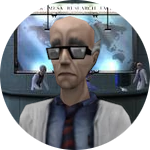
\includegraphics[width=3cm]{opening/resources/about/kleiner.png} & \vspace{-0.5mm} {\large \thesisAuthor} 
        \newline A short paragraph about you and how handsome and hard-working you are. Brag about your work, awards, publications and merits. The glory is yours! Congratulations. The Lorem ipsum dolor sit amet, consectetur adipiscing elit. Integer tempus quis elit id sagittis. Cras tincidunt nisi at tellus luctus, et congue dolor posuere. Aliquam suscipit felis sit amet lacus ultrices aliquet. Sed sagittis ultrices nisi, vel elementum elit dignissim non. 
        \vspace{2mm} 
        \newline
        \href{https://orcid.org/}{  % Link to your orcid
            \icon{\faOrcid}{10}{orcid-green}
        }
        \href{https://www.linkedin.com/}{  % Link to your linkedin
            \icon{\faLinkedinIn}{10}{linkedin-blue}
        }
        \href{https://github.com/}{  % Link to your github
            \icon{\faGithub}{10}{github-black}
        }
        \href{https://twitter.com/}{  % Link to your twitter
            \icon{\faTwitter}{10}{twitter-blue}
        }
        \href{mailto:example@domain.org}{  % Your E-mail
            \icon{\faEnvelope}{10}{email-red}
        }
        \href{https://t.me/}{  % Link to your telegram
            \icon{\faTelegramPlane}{10}{telegram-blue}
        }
    \end{tabular}
    
    \vspace{10mm}
    
    \noindent
    \begin{tabular}{p{3.5cm} p{11.5cm}}
        \vspace{0mm} 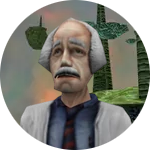
\includegraphics[width=3cm]{opening/resources/about/coomer.png} & \vspace{-0.5mm} {\large \thesisTutor} 
        \newline What a big fish you've got yourself. Show off your tutor. Now that's a job well done. Lorem ipsum dolor sit amet, consectetur adipiscing elit. Integer tempus quis elit id sagittis. Cras tincidunt nisi at tellus luctus, et congue dolor posuere. Aliquam suscipit felis sit amet lacus ultrices aliquet. Sed sagittis ultrices nisi, vel elementum elit dignissim non. Fusce faucibus ex at massa ultrices elementum.
        \vspace{2mm} 
        \newline
        \href{https://orcid.org/}{  % Link to your orcid
            \icon{\faOrcid}{10}{orcid-green}
        }
        \href{https://www.linkedin.com/}{  % Link to your linkedin
            \icon{\faLinkedinIn}{10}{linkedin-blue}
        }
        \href{https://github.com/}{  % Link to your github
            \icon{\faGithub}{10}{github-black}
        }
        \href{https://twitter.com/}{  % Link to your twitter
            \icon{\faTwitter}{10}{twitter-blue}
        }
        \href{mailto:example@domain.org}{  % Your E-mail
            \icon{\faEnvelope}{10}{email-red}
        }
        \href{https://t.me/}{  % Link to your telegram
            \icon{\faTelegramPlane}{10}{telegram-blue}
        }
    \end{tabular}
    
\endgroup





%%%%%%%%%%%%%%%%%%%%%%%%%%%%%%%%%%%%%%%%%%%%%%%%%%%%%%%%%%%%%%%%%%%%%%%%%%%%%%%%%%%%%%%%%%%%
% how to cite this work

% Listings workaround to include the background in broken lines

% \begin{verbatimwrite}{cite.txt}
% @mastersthesis{citeKey,
%     author  = "(*@{\thesisAuthor}@*) and (*@{\thesisTutor}@*)",
%     title   = "(*@{\thesisTitle}@*)",
%     school  = "(*@{\thesisSchool}@*)",
%     year    = "(*@{\thesisYear}@*)",
%     month   = "(*@{\thesisMonth}@*)",
%     address = "(*@{\thesisAddress}@*)"
% }
% \end{verbatimwrite}


\begingroup

\vspace*{\fill}

\small
\setlength\tabcolsep{0pt}
\renewcommand*{\arraystretch}{1.2}
{\noindent\large  Cite this work:}

% \begin{mdframed}[backgroundcolor=listing-background,hidealllines=true]
\vspace*{2mm}
% \lstinputlisting[style=cite, nolol]{./cite.txt}

\newwrite\tempfile
\immediate\openout\tempfile=cite.txt
\immediate\write\tempfile{%
@mastersthesis{citeKey,^^J
author  = "\thesisAuthor \space and \thesisTutor",^^J
title   = "\thesisTitle",^^J
school  = "\thesisSchool",^^J
year    = "\thesisYear",^^J
month   = "\thesisMonth",^^J
address = "\thesisAddress",^^J
type = "\thesisType"^^J
}
}
\immediate\closeout\tempfile

% Does not work because escapes are inside strings
% \begin{minted}{bibtex}
% @mastersthesis{citeKey,
%     author  = "¢{\thesisAuthor}¢ and ¢{\thesisTutor}¢",
%     title   = "¢{\thesisTitle}¢",
%     school  = "¢{\thesisSchool}¢",
%     year    = "¢{\thesisYear}¢",
%     month   = "¢{\thesisMonth}¢",
%     address = "¢{\thesisAddress}¢"
% }
% \end{minted}

\inputminted[style=algol_nu]{bibtex}{./cite.txt}
% \end{mdframed}


\endgroup

\newpage
\thispagestyle{empty}


\cleardoublepage
\phantomsection
\begin{center}
    \textbf{\large DECLARATION}
\end{center}


I declare that have produced the Master’s thesis \textbf{\thesisTitle} independently and without improper external assistance and that I have identified all
word-for-word quotations of other authors, as well as comments based closely on other authors’ ideas, and I have listed the relevant sources.


I am aware that, unless agreed otherwise, the Master’s thesis  produced under supervision represents a group achievement and forms part of the overall
research of the supervising institution. As a result, none of the co-authors (e.g. authors of text, creative project staff, co-supervisors) may use passages
from the thesis for commercial purposes or make them accessible to third parties without the (written) approval of all those involved due to reasons of copyright.
Particular note must be taken of the Arbeitnehmererfindergesetz (German Employee Invention Act), according to which pre-publication of patent-related content is prohibited.




\vspace*{2cm}
\noindent
\begin{minipage}[t]{0.5\textwidth}
    \textbf{Date:} \today
\end{minipage}%
\begin{minipage}[t]{0.5\textwidth}
    \flushright
    \textbf{Signature:} \underline{\hspace{4cm}}
\end{minipage}

% Abstract
% 
%            ,,                                        
%          `7MM            _.o9                                
%            MM                                             
%  ,6"Yb.    MM  ,p6"bo   ,6"Yb.  M"""MMV  ,6"Yb.  `7Mb,od8 
% 8)   MM    MM 6M'  OO  8)   MM  '  AMV  8)   MM    MM' "' 
%  ,pm9MM    MM 8M        ,pm9MM    AMV    ,pm9MM    MM     
% 8M   MM    MM YM.    , 8M   MM   AMV  , 8M   MM    MM     
% `Moo9^Yo..JMML.YMbmd'  `Moo9^Yo.AMMmmmM `Moo9^Yo..JMML.   
% 
% 
% Free and Open-Source template for academic works
% https://github.com/dpmj/alcazar

\newpage

\clearpage
\cleardoublepage
\phantomsection

\pagestyle{plain}

\phantomsection
\addcontentsline{toc}{chapter}{Abstract}

{\noindent \large \textbf{\thesisTitle}}\\

{\noindent \textbf{\textsc{Keywords:}}}

{\noindent \thesisKeywords}\\


{\noindent \textbf{\textsc{Abstract:}}}

\noindent Abstract in the same language as the main text. Lorem ipsum dolor sit amet, consectetur adipiscing elit. Integer tempus quis elit id sagittis. Cras tincidunt nisi at tellus luctus, et congue dolor posuere. Aliquam suscipit felis sit amet lacus ultrices aliquet. Sed sagittis ultrices nisi, vel elementum elit dignissim non. Fusce faucibus ex at massa ultrices elementum. Nullam ullamcorper lorem sit amet facilisis cursus. Suspendisse non erat non justo porta placerat. Morbi porttitor dictum molestie. Sed vitae iaculis libero. Suspendisse in gravida lacus, tempor ultrices nibh. Nam consequat scelerisque porttitor.

Nulla elementum orci in dolor dapibus, ac facilisis sem ultrices. Nullam eleifend id eros sed luctus. Maecenas arcu ipsum, scelerisque id lorem in, placerat posuere tellus. Etiam gravida velit sed arcu viverra dapibus. Mauris vitae augue dapibus, molestie justo eget, condimentum ipsum. Nulla tristique mi eget semper luctus. Etiam commodo vestibulum vulputate. Etiam quis sapien dolor. Nunc tristique eu lacus quis ullamcorper. Sed volutpat rutrum vehicula. Donec nunc nisl, suscipit in faucibus vitae, tristique eu risus. Nulla facilisis augue eget interdum rutrum. Aliquam sem nunc, fermentum sed urna ac, faucibus interdum nisi.

Proin a condimentum nibh. Praesent vulputate tellus vel metus rutrum, non luctus mi sollicitudin. Nam ac tellus ut eros sollicitudin luctus at ac mi. Vestibulum mollis nec nisi a laoreet. Proin neque tortor, placerat nec suscipit sit amet, ullamcorper in sem. Fusce faucibus ultrices cursus. Maecenas scelerisque mauris diam, at volutpat nisi porta vitae. Sed at ipsum et leo cursus varius eu eu lectus. Class aptent taciti sociosqu ad litora torquent per conubia nostra, per inceptos himenaeos. Ut felis ipsum, imperdiet rhoncus orci ac, consectetur luctus nisl. Cras aliquet elementum tellus ullamcorper malesuada. Integer purus est, pharetra eu ullamcorper quis, imperdiet non turpis.

In vestibulum faucibus ligula eget blandit. Donec eget cursus risus, quis suscipit justo. Curabitur efficitur, dolor nec pulvinar pellentesque, lectus eros hendrerit nisi, in aliquet erat nunc non ipsum. Curabitur felis nunc, viverra nec quam ultrices, suscipit condimentum nibh. Nam faucibus felis hendrerit imperdiet maximus. Curabitur tincidunt porttitor lectus quis feugiat. Sed imperdiet bibendum mi.

Nullam quis lacus vel ante feugiat efficitur id ut quam. Pellentesque commodo elit nec urna gravida maximus. Suspendisse ut risus eu ipsum porta porta ac et orci. Donec dictum ligula sodales, euismod est sed, semper libero. In blandit, nulla et elementum pharetra, mi nunc sagittis tellus, sit amet scelerisque magna elit ac sapien. Curabitur ipsum dui, pretium a maximus id, varius gravida nisl. Sed vitae mattis elit, vitae hendrerit lorem. 



%% ADDITIONAL LANGUAGES
% Translate your title and keywords to match the language


\newpage
\thispagestyle{empty}

\clearpage
\cleardoublepage
\phantomsection

\pagestyle{plain}

{\noindent \large \textbf{\thesisTitle}}\\

{\noindent \textbf{\textsc{Palabras clave:}}}

{\noindent \thesisKeywords}\\


{\noindent \textbf{\textsc{Resumen:}}}

\noindent Resumen en un idioma diferente - Abstract in a different language.
Lorem ipsum dolor sit amet, consectetur adipiscing elit. Integer tempus quis elit id sagittis. Cras tincidunt nisi at tellus luctus, et congue dolor posuere. Aliquam suscipit felis sit amet lacus ultrices aliquet. Sed sagittis ultrices nisi, vel elementum elit dignissim non. Fusce faucibus ex at massa ultrices elementum. Nullam ullamcorper lorem sit amet facilisis cursus. Suspendisse non erat non justo porta placerat. Morbi porttitor dictum molestie. Sed vitae iaculis libero. Suspendisse in gravida lacus, tempor ultrices nibh. Nam consequat scelerisque porttitor.

Nulla elementum orci in dolor dapibus, ac facilisis sem ultrices. Nullam eleifend id eros sed luctus. Maecenas arcu ipsum, scelerisque id lorem in, placerat posuere tellus. Etiam gravida velit sed arcu viverra dapibus. Mauris vitae augue dapibus, molestie justo eget, condimentum ipsum. Nulla tristique mi eget semper luctus. Etiam commodo vestibulum vulputate. Etiam quis sapien dolor. Nunc tristique eu lacus quis ullamcorper. Sed volutpat rutrum vehicula. Donec nunc nisl, suscipit in faucibus vitae, tristique eu risus. Nulla facilisis augue eget interdum rutrum. Aliquam sem nunc, fermentum sed urna ac, faucibus interdum nisi.

Proin a condimentum nibh. Praesent vulputate tellus vel metus rutrum, non luctus mi sollicitudin. Nam ac tellus ut eros sollicitudin luctus at ac mi. Vestibulum mollis nec nisi a laoreet. Proin neque tortor, placerat nec suscipit sit amet, ullamcorper in sem. Fusce faucibus ultrices cursus. Maecenas scelerisque mauris diam, at volutpat nisi porta vitae. Sed at ipsum et leo cursus varius eu eu lectus. Class aptent taciti sociosqu ad litora torquent per conubia nostra, per inceptos himenaeos. Ut felis ipsum, imperdiet rhoncus orci ac, consectetur luctus nisl. Cras aliquet elementum tellus ullamcorper malesuada. Integer purus est, pharetra eu ullamcorper quis, imperdiet non turpis.

In vestibulum faucibus ligula eget blandit. Donec eget cursus risus, quis suscipit justo. Curabitur efficitur, dolor nec pulvinar pellentesque, lectus eros hendrerit nisi, in aliquet erat nunc non ipsum. Curabitur felis nunc, viverra nec quam ultrices, suscipit condimentum nibh. Nam faucibus felis hendrerit imperdiet maximus. Curabitur tincidunt porttitor lectus quis feugiat. Sed imperdiet bibendum mi.

Nullam quis lacus vel ante feugiat efficitur id ut quam. Pellentesque commodo elit nec urna gravida maximus. Suspendisse ut risus eu ipsum porta porta ac et orci. Donec dictum ligula sodales, euismod est sed, semper libero. In blandit, nulla et elementum pharetra, mi nunc sagittis tellus, sit amet scelerisque magna elit ac sapien. Curabitur ipsum dui, pretium a maximus id, varius gravida nisl. Sed vitae mattis elit, vitae hendrerit lorem. 




% Publications
% 
%            ,,                                        
%          `7MM            _.o9                                
%            MM                                             
%  ,6"Yb.    MM  ,p6"bo   ,6"Yb.  M"""MMV  ,6"Yb.  `7Mb,od8 
% 8)   MM    MM 6M'  OO  8)   MM  '  AMV  8)   MM    MM' "' 
%  ,pm9MM    MM 8M        ,pm9MM    AMV    ,pm9MM    MM     
% 8M   MM    MM YM.    , 8M   MM   AMV  , 8M   MM    MM     
% `Moo9^Yo..JMML.YMbmd'  `Moo9^Yo.AMMmmmM `Moo9^Yo..JMML.   
% 
% 
% Free and Open-Source template for academic works
% https://github.com/dpmj/alcazar


% Add here your Publications.
% Depends on Biblatex and Biber for multiple bibliographies.

\newpage
\pagestyle{empty}

\clearpage
\cleardoublepage
\phantomsection

\pagestyle{empty}

% \phantomsection
% \addcontentsline{toc}{chapter}{Publications}


\begin{refsection}

    \nocite{own-article-1, own-article-2, own-article-3}

    \defbibnote{pre-note}{
        \noindent The {\thesisDegree} candidate, {\thesisAuthor}, has co-authored the following publications with Prof. {\thesisTutor} et al. The articles come as a result of the research activities carried out during the {\thesisType}. The candidate is the corresponding author in two of the three publications listed below:
    }
    \defbibnote{post-note}{
        \noindent Note: \cite{own-article-3} is not yet published.
    }

    \printbibliography[heading=bibintoc,  % Title in Table of contents
                       title={Publications},  % Title
                       prenote=pre-note,  % Text before bibliography
                       postnote=post-note]  % Text after bibliography

\end{refsection}


  % Optional: comment this line if you don't need it

% Acknowledgements
% % 
%            ,,                                        
%          `7MM            _.o9                                
%            MM                                             
%  ,6"Yb.    MM  ,p6"bo   ,6"Yb.  M"""MMV  ,6"Yb.  `7Mb,od8 
% 8)   MM    MM 6M'  OO  8)   MM  '  AMV  8)   MM    MM' "' 
%  ,pm9MM    MM 8M        ,pm9MM    AMV    ,pm9MM    MM     
% 8M   MM    MM YM.    , 8M   MM   AMV  , 8M   MM    MM     
% `Moo9^Yo..JMML.YMbmd'  `Moo9^Yo.AMMmmmM `Moo9^Yo..JMML.   
% 
% 
% Free and Open-Source template for academic works
% https://github.com/dpmj/alcazar


% Add here your Acknowledgements. 
% This section is pretty free: free format, in one or various languages, etc.


\newpage
\thispagestyle{empty}

\clearpage
\cleardoublepage
\phantomsection

\pagestyle{plain}

\phantomsection
\addcontentsline{toc}{chapter}{Acknowledgements}


\vspace*{\fill}

\begin{center}
    \large \textbf{\textsc{Acknowledgements}}
\end{center}

@TODO start from here [usman]



% Dedication
% To whom do you dedicate the thesis? Or maybe include a quote, poem, etc. Free space for yourself.
% Delete if you are too manly for these things
% % 
%            ,,                                        
%          `7MM            _.o9                                
%            MM                                             
%  ,6"Yb.    MM  ,p6"bo   ,6"Yb.  M"""MMV  ,6"Yb.  `7Mb,od8 
% 8)   MM    MM 6M'  OO  8)   MM  '  AMV  8)   MM    MM' "' 
%  ,pm9MM    MM 8M        ,pm9MM    AMV    ,pm9MM    MM     
% 8M   MM    MM YM.    , 8M   MM   AMV  , 8M   MM    MM     
% `Moo9^Yo..JMML.YMbmd'  `Moo9^Yo.AMMmmmM `Moo9^Yo..JMML.   
% 
% 
% Free and Open-Source template for academic works
% https://github.com/dpmj/alcazar

\newpage
\thispagestyle{empty}

\clearpage
\cleardoublepage
\phantomsection

\thispagestyle{empty}

\phantomsection
\addcontentsline{toc}{chapter}{Dedication}



\vspace*{\fill}

\begin{flushright}

\textit{\large
\noindent ``Y así, mi señor, es como sabemos que\\
la Tierra tiene forma de plátano''\\ 
}

\vspace{0.5cm}

\textbf{Sir Bedevere el Sabio}\\

\vspace{0.3cm}

Interpretado por \textsc{Terry Jones}\\

\vspace{0.2cm}

{
\noindent En \textit{Monty Python y los caballeros\\
de la mesa cuadrada,} 1975\\
}

\vspace{2cm}
\end{flushright}



\vspace*{\fill}



% ------------------------------------------------------------------------------
% TABLES OF CONTENTS

\newpage
\thispagestyle{empty}

\clearpage
\cleardoublepage
\phantomsection

\pagestyle{plain}


\begingroup

% Greatly compress space used by TOC, LOF and LOT
\renewcommand{\baselinestretch}{1}  % less spacing
\small  % smaller font size
\setlength{\parskip}{0mm}  % Paragraph skip 0mm


% List of Contents
{
    \tableofcontents

    \addcontentsline{toc}{chapter}{Table of contents}
}

% List of Figures
{
    \listoffigures
    \addcontentsline{toc}{chapter}{List of figures}
}

% List of Tables
{
    \listoftables
    \addcontentsline{toc}{chapter}{List of tables}
}

% List of Listings -- uncomment if necessary
{
    % \listoflistings
    % \addcontentsline{toc}{chapter}{List of listings}

    % \listof{lstlisting}{Code listings} % old code
}

\endgroup

% END OPENING
% ------------------------------------------------------------------------------


